\def\SigmaBlob{plot[smooth cycle,tension=0.7] coordinates {(-3.2,0.1) (-2.6,0.9) (-1.2,1.7) (0.8,1.9) (2.6,1.5) (3.3,0.4) (2.8,-0.9) (1.0,-1.5) (-1.4,-1.4) (-3.0,-0.8)}}

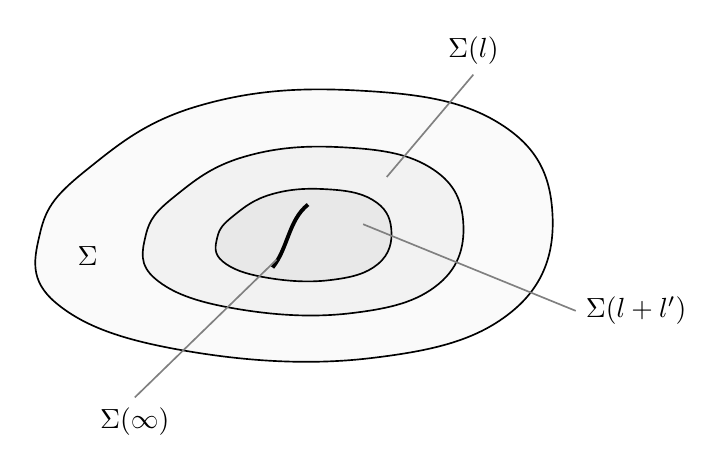
\begin{tikzpicture}[line width=0.6pt]
  \draw[fill=gray!4] \SigmaBlob;
  \begin{scope}[scale=0.62,xshift=0.2cm]\draw[fill=gray!10] \SigmaBlob;\end{scope}
  \begin{scope}[scale=0.34,xshift=0.4cm]\draw[fill=gray!18] \SigmaBlob;\end{scope}
  \draw[line width=1.4pt] (-0.25,-0.35) .. controls (-0.05,-0.1) and (-0.05,0.25) .. (0.2,0.45);
  \node at (-2.6,-0.2) {$\Sigma$};
  \draw[gray] (1.2,0.8) -- (2.3,2.1) node[above,black] {$\Sigma(l)$};
  \draw[gray] (0.9,0.2) -- (3.6,-0.9) node[right,black] {$\Sigma(l+l')$};
  \draw[gray] (-0.2,-0.25) -- (-2.0,-2.0) node[below,black] {$\Sigma(\infty)$};
\end{tikzpicture}
